\subsection{Performance}

\begin{frame}
\begin{center}
\frametitle {Performance Analyse}
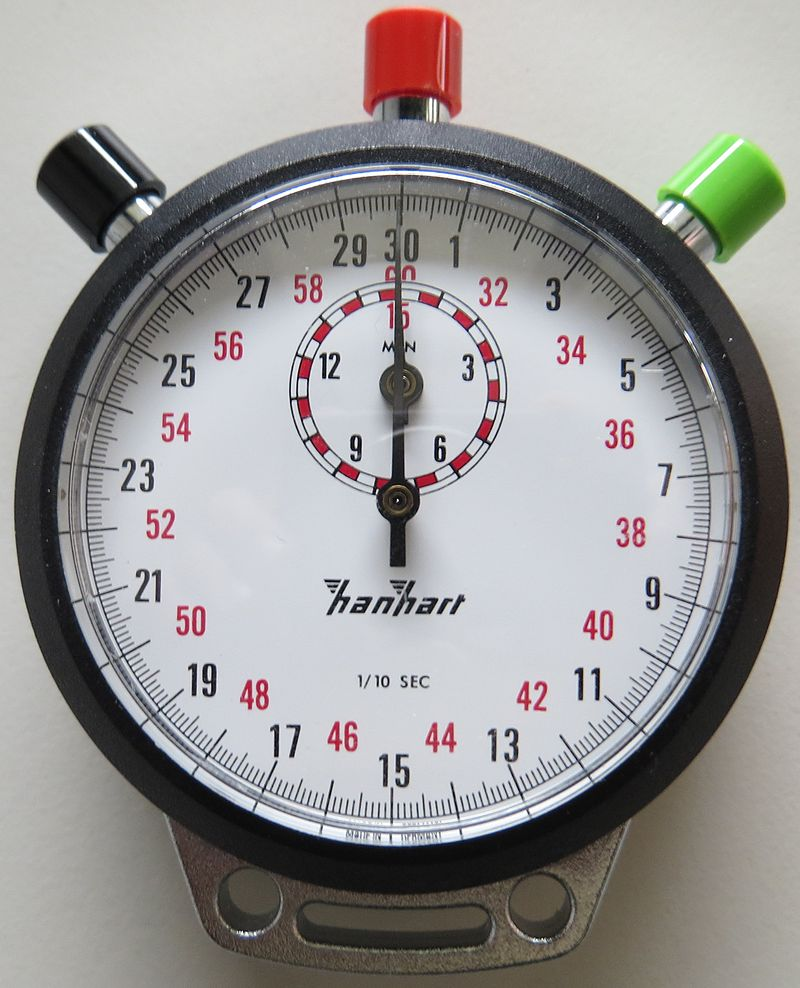
\includegraphics[scale=0.4]{performance/clock}
\end{center}
\end{frame}

\begin{frame}
\frametitle{Rechner Phase 1}
\begin{itemize}
	\item Chevalblanc
	\item Virtuelle Maschine (QEMU 1.1.2 mit KVM Support)
	\item 1 CPU Kern - 2.00 GHz (64 bit)
	\item 2 GB RAM
	
\end{itemize}
\end{frame}

\begin{frame}
\frametitle{Websocket-Verbindungen}
	\begin{center}
		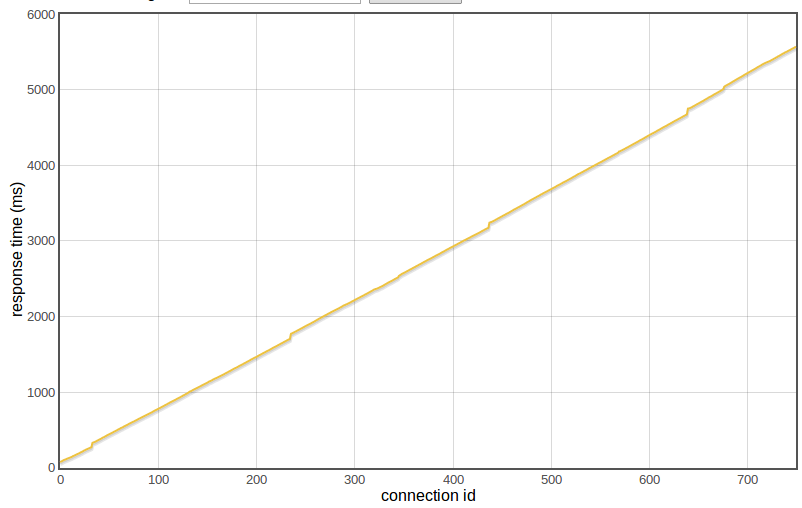
\includegraphics[scale=0.3]{performance/750-sockets.png}
		% 500 gleichzeitig eingeleitete Verbindungen
		% 500 maximum des Laptops
		% maximale CPU Auslastung von etwa 15%
		% Reiner Verbindungsaufbau
		% Websocket idle bei 500 Verbindungen ist bei < 1% CPU
		% sequentielle Abarbeitung der Verbindungen
		% => Mehr User = linearer Latenzanstieg
		% 1 Thread behandelt websockets
		% => Multithreading (start simulation etc)
		%TODO Berechne durchschnittssteigerung
		%TODO Einfluss der Simulation
	
	\end{center}
\end{frame}

\begin{frame}
\frametitle{StdIn vs StdOut}
\begin{center}
	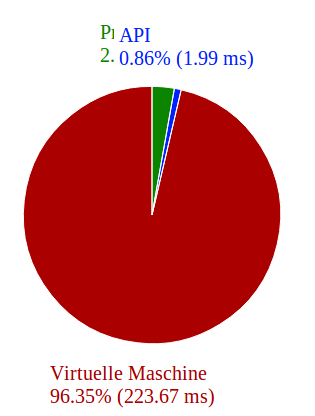
\includegraphics[scale=0.3]{performance/100-turns.png}
	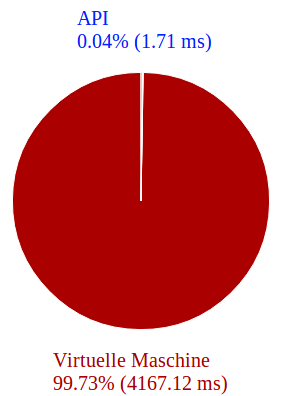
\includegraphics[scale=0.3]{performance/100-looks.png}
	% 100*look
	% 80ms pro look
	% turn: 0.007824740000000002ms
	% Preprozessor: 2.79% (6.48 ms), Pendelt zwischen 6 und 12ms
\end{center}

\end{frame}

\begin{frame}
	
	
	\begin{center}
	
	\begin{tabular}{c|c}
	Parallele Instanzen & Operationen\\
	\hline% countOps, Beeinflussung
	 1	&562\\
	5	&562\\
	6	&564\\
	7	&567\\
	8	&557\\
	9	&549\\
	10	&545\\
	50&	300\\
	100 &	228\\
	\end{tabular}
	
	\end{center}
	

\end{frame}

\begin{frame}	
	\begin{center}
	
	\begin{tabular}{c|c}
	Parallele Instanzen & CPU Auslastung\\
	\hline
	 1	& 8\%\\
	5	& 28\%\\
	50	& 65\%\\
	100	& 60\%\\
	200	& 46\%\\
	\end{tabular}
	
	\end{center}
\end{frame}

\begin{frame}
\begin{center}
\begin{scriptsize}
\LARGE Ausblick \& Fazit

\end{scriptsize}
\end{center}
\end{frame}
